% ------------------------------------------------------------------------------
% Resultados
% ------------------------------------------------------------------------------

\chapter{Resultados}

A simulação dos 10 caminhantes após realizar 10000 passos pode ser visualizada no gráfico abaixo. O gráfico mostra a posição do caminhante a cada passo realizado. Todos os caminhantes parte da origem na esquerda e a a ultima marcação mais à direita mostra a posição final. 

\begin{figure}[!htb]
  \centering
  \caption{Simulação caminhantes}
  \label{simulacao_caminhates}
  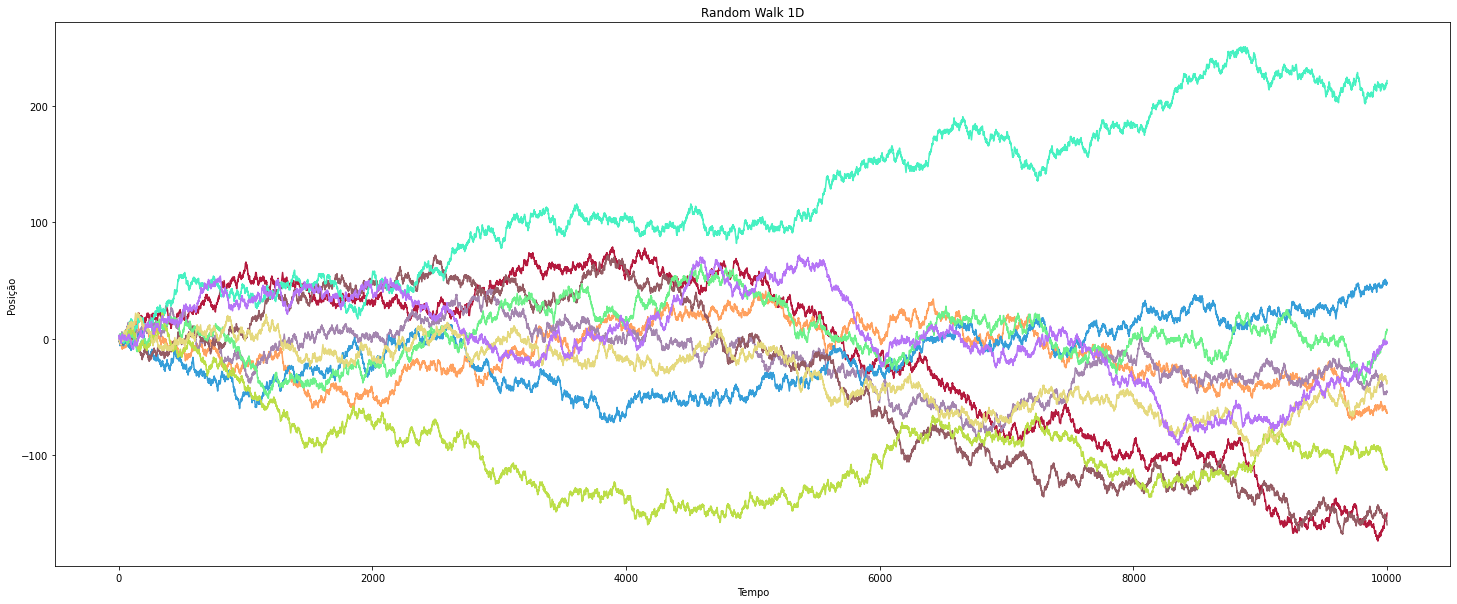
\includegraphics[width=1\textwidth]{figuras/output_0.png}
\end{figure}

Calculamos o desvio médio quadrático $R^{2}$ para todos os 10 caminhantes e desenhamos um gráfico com a escala log-log. 

\begin{figure}[!htb]
  \centering
  \caption{Desvio médio quadrático log-log}
  \label{devio_medio}
  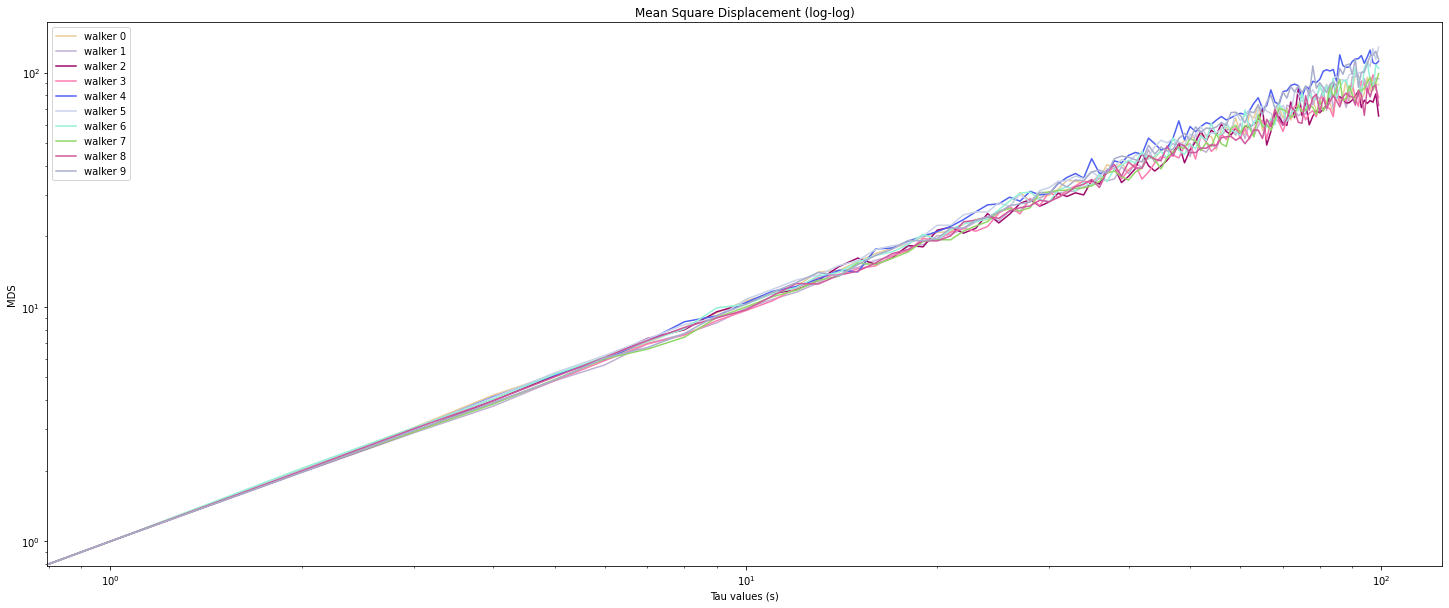
\includegraphics[width=1\textwidth]{figuras/output_1.png}
\end{figure}

Para ter uma série de dados única para ajustar uma função de lei de potência, fizemos a média dos resultados obtidos do $R^{2}$ de todos os caminhantes. A curva das médias pode ser vista no gráfico abaixo.

\begin{figure}[!htb]
  \centering
  \caption{Média do desvio médio quadrático log-log}
  \label{media_devio_medio}
  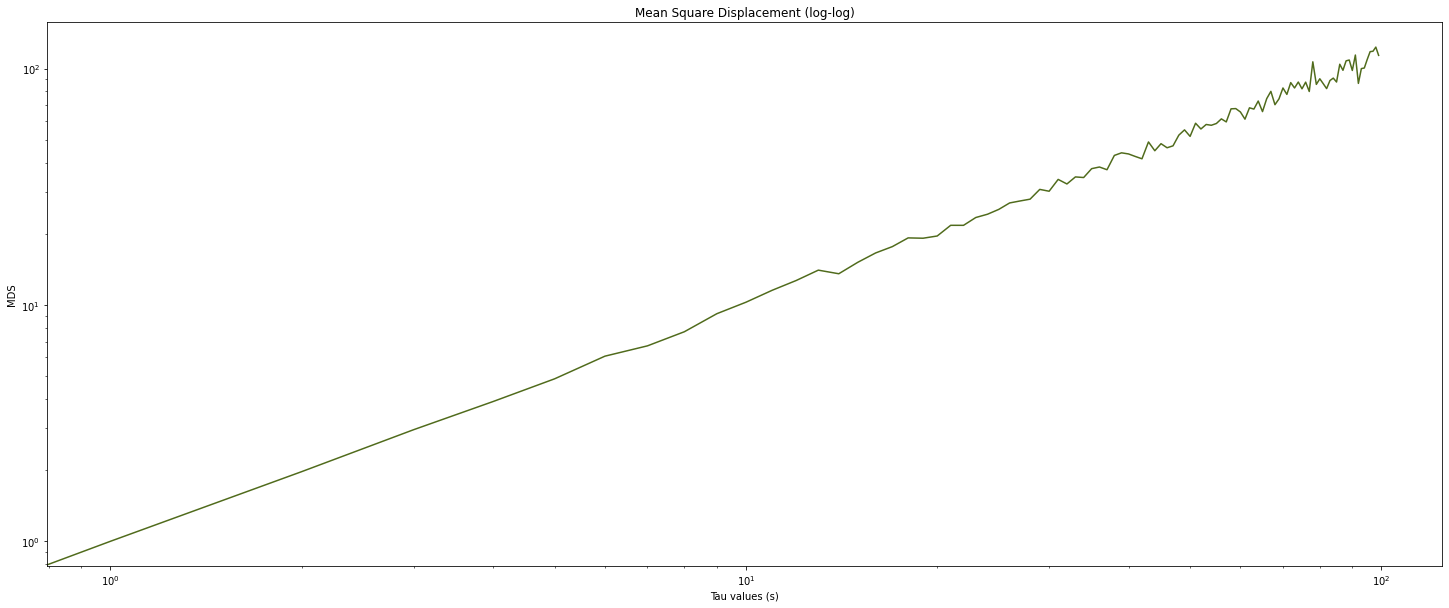
\includegraphics[width=1\textwidth]{figuras/output_2.png}
\end{figure}

Ajustamos a uma função de lei de potência para a série de dados e obtemos uma função com parâmetros:
$ a: 1.0632266820499991 $ e $ b: 0.9836350285341431 $. 

$$ y = 1.063226682049999x^{0.9836350285341431} $$

Desenhamos um novo gráfico com a serie de dados e com a função da lei de potência para visualizar a qualidade do ajuste.

\begin{figure}[!htb]
  \centering
  \caption{Lei de potência}
  \label{curva_lei_potencia}
  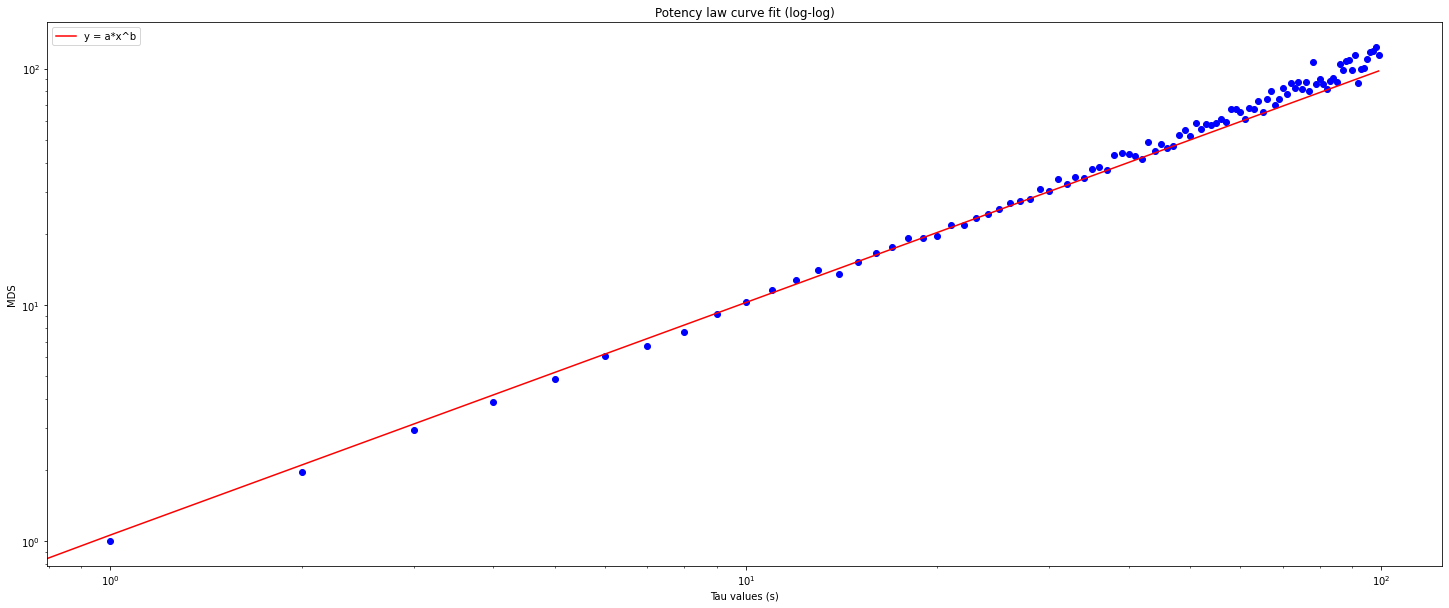
\includegraphics[width=1\textwidth]{figuras/output_3.png}
\end{figure}

Para verificar que a simulação respeita o teorema central do limite, desenhamos um histograma com a posição final de 1000 caminhantes e utilizamos o histograma para ajustar uma função gaussiana. O gráfico abaixo mostra o resultado obtido. 

\begin{figure}[!htb]
  \centering
  \caption{Histograma}
  \label{histograma}
  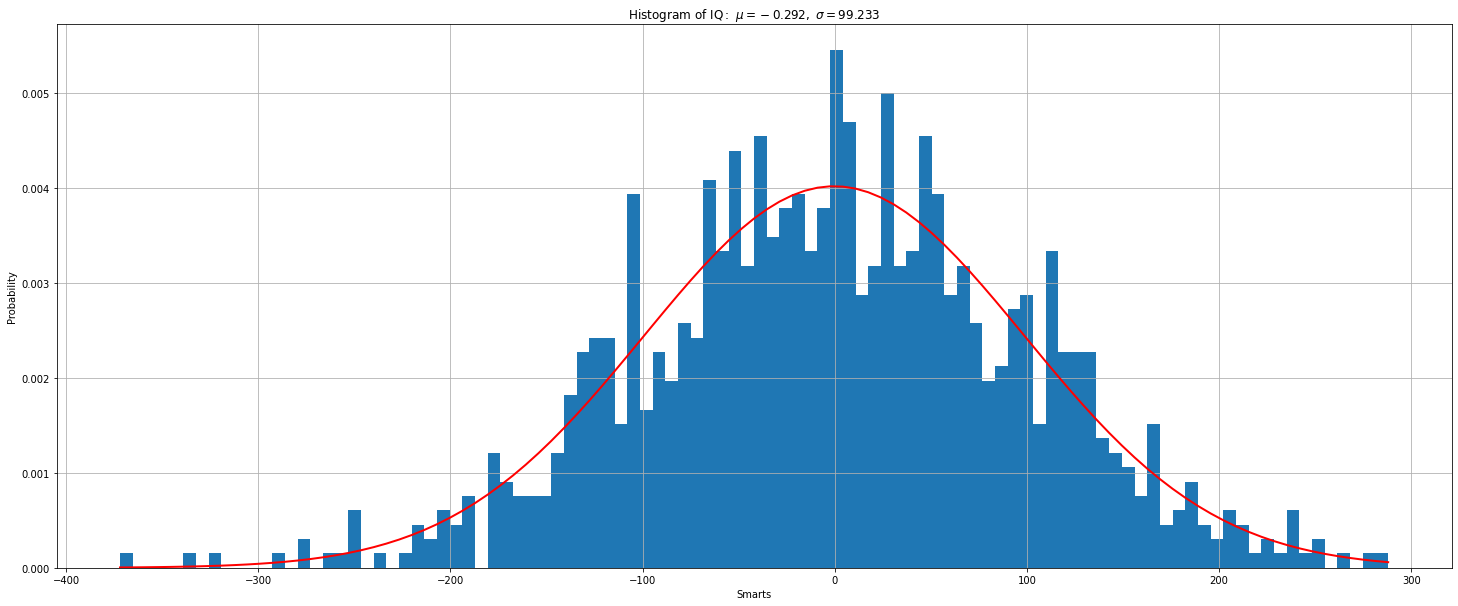
\includegraphics[width=1\textwidth]{figuras/output_4.png}
\end{figure}

\section{Discussão}
\label{sec_discussao_resultados}

O gráfico de posição x tempo é uma ótima forma de visualizar comparativamente as diversas interações da simulação do random walk. Com ele podemos visualizar lado a lado a posição de cada simulação desde a origem até a posição final. O formato final das curvas nos permite adquirir a intuição sobre o comportamento de uma entidade se movendo de maneira aleatória.

Ao calcular o desvio médio quadrático e desenhar o gráfico na escala log-log. Vemos que as curvas são aproximadamente lineares. os gráfico log-log mostram linhas retas para funções exponenciais, variando a inclinação da reta de acordo com o expoente. 

Para identificar o expoente da função fazemos o ajuste de uma função de lei de potência. A função ajustada tem expoente 1, o que indica que o random walk implementado é realmente um caminhante aleatório.

O gráfico da função ajustada e da série de dados mostra que o ajuste feito realmente aproxima os valores da série.

O gráfico do histograma mostra o resultado da posição final de 1000 simulação. A posição final foi agrupada em blocos de 100 para cada coluna do histograma. Sobre o histograma desenhamos uma gaussiana (curva em formato de sino). Foi necessário normalizar o histograma antes de ajustar a gaussiana ajustada.
